\chapter{Introduction}


The ever growing organisations involved in search engines, social networking as well as applications for mobile devices, require efficient analysis of the massive collections of the data generated, which is achieved using thousands of commodity servers, resulting in the growing trend of \textit{Big Data Analytics} \cite{mcafee2012big}. Big data applications process data by distributing it across the data centre clusters, and after each piece has been analysed in parallel, the final data set is transferred and merged across the data centre network.

To support such communication patterns, data centre topologies make use of \textit{multi-rooted tree} topologies in order to achieve higher speed links among the clusters and bypass the limitations caused by \textit{limited port densities} in commodity switches \cite{al2010hedera}. The goal of \textit{multi-rooted tree} topologies is to enable efficient communication among the network hosts by increasing the number of paths that interconnect them, thereby creating redundancy. Path multiplicity in \textit{multi-rooted tree topologies} is achieved by horizontal scaling of hosts \cite{al2008scalable, greenberg2009vl2, guo2008dcell,guo2009bcube} in order to cater to the increasing processing demands of big data applications.

Traditional network traffic routing protocols are designed for much simplistic communication patterns and topologies, with limited paths between host destination pairs, where the small number of redundant paths are used for fault tolerance, making them not suitable to be used for routing traffic in topologies with path diversity. Additional obstacles in routing of big data application traffic are possible escalation in network traffic volumes, multiplicity of traffic patterns and high duration of data processing jobs. As a result, various studies \cite{al2010hedera, greenberg2009vl2,guo2008dcell} have highlighted that the network is a bottleneck in the performance of big data applications. 

A significant amount of research \cite{das2013transparent, wang2012programming, al2010hedera, narayan2012hadoop, neves2014pythia, wette2015hybridte} has been conducted with the sole purpose of optimizing traffic in a data centre network for large-scale data analysis by devising new flow scheduling mechanisms and programming the entire network stack, so as to maximize throughput in the network, enabling better performance of big data applications. All work done in this field employs the emergent technology of Software-Defined Networking (SDN), in order to configure the network in accordance with big data application communication patterns.  

\begin{figure}[!ht]
\centerline{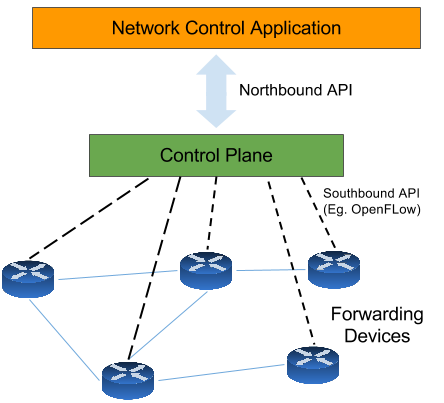
\includegraphics[scale=0.50]{SDNOverview.png}}
\caption{Fundamental abstractions of SDN.}
\label{Sec:SDNOverview}
\end{figure}

SDN allows the control of all forwarding devices in the network from a global vantage point; it achieves this by separation of the control plane from the data plane of the forwarding devices, enabling centralized control of the network \cite{mckeown2011sdn}. Moreover, it maintains the global state of the network and is responsible for the routing protocols being used in the network, enabling prototyping of new flow scheduling mechanisms. A high level overview of the SDN architecture is illustrated in Figure \ref{Sec:SDNOverview}. SDN allows for network programmability by installing flows in the switches, based on control logic that sits in a centralized controller which has a global view of the network. Hence, network applications can be developed which aim to maximize throughput by creating a tight-coupling between network flow scheduling and application communication patterns.  

Consequently, using SDN, the data centre network can be optimized to handle the traffic patterns of big data applications in topologies with path diversity, without being limited by traditional routing protocols which are insufficient to handle such communication patterns. 

\section{Project Motivation}

The motivation behind the current project is to device a flow scheduling approach in accordance with \textit{big data} application patterns, in particular MapReduce \cite{dean2008mapreduce}, which is \textit{proactive} in nature, so that the data centre network achieves maximum throughput and the application performs better. Existing research focuses on dynamic configuration of data centre networks by \textit{reactively} scheduling flows at application runtime. Our goal is to investigate if there are performance gains in terms of the total bisection bandwidth achieved by hosts running big data applications in the network, when the network is optimized \textit{proactively} based on application traffic patterns. 

By taking a global view of the network using SDN, we preconfigure the scheduling system in order to avoid bottlenecks and minimize control traffic overhead in the network. We use Hadoop \cite{HadoopWeb} as the application for proactive network integration due to it's widespread use and popularity. 

\section{Project Aims}
We propose a \textit{Proactive} approach for the configuration of a data centre network, which installs flow rules in the network before the big data application starts. In particular, we intend to 
\begin{itemize}
\item Determine whether there is an increase in the total bisection bandwidth achieved by the hosts in the network when flows are scheduled \textit{proactively}.  
\item Investigate the effectiveness of \textit{proactive} network configuration by comparing the Hadoop job completion times with \textit{reactive} flow scheduling approaches and static Equal Cost Multi-Path (ECMP \cite{hopps2000analysis}) routing.
\item Determine if there is an inverse correlation between total bisection bandwidth achieved and Hadoop job completion times for different flow scheduling strategies.  
\end{itemize}
\section{Project Approach}
We present a design of our \textit{Proactive} flow scheduler based on python, which leverages the flow scheduling decisions made by Global First-Fit \cite{al2010hedera} flow scheduling algorithm. Subsequently, we analyse the performance of our \textit{Proactive} flow scheduler against ECMP routing and Global First-Fit flow scheduling on an emulation based testbed.
\section{Document Structure}

Chapter \ref{chap:State} explores the current state-of-the-art in efforts to optimize data centre network traffic for big data applications using SDN, and the emulators used for prototyping novel network control logic. Chapter \ref{chap:Background} provides background for the project, explaining the working of MapReduce and its implementation in Hadoop, subsequently describing current state-of-the-art in data centre topologies such as the \textit{fat-tree topology} \cite{al2008scalable}, and finally providing an overview of ECMP routing and Global First-Fit flow scheduling which are used for evaluating our \textit{Proactive} flow scheduling. Chapter \ref{chap:design} describes the design of our \textit{Proactive} flow scheduler and gives a functional architectural overview of our experimental setup. The actual implementation of the design is described in Chapter \ref{chap:Implmentation}. Chapter \ref{chap:eval} details the benchmark tests used for evaluating our \textit{Proactive} flow scheduler against ECMP routing and Global First-Fit flow scheduling and provides a brief analysis on the results obtained. Finally, Chapter \ref{chap:conc} contains our concluding remarks.  
